\subsubsection{Reference Forms}
\label{subsec:referenceForms}
The basic structure of our web application was described in the previous
sections. This was the part of the application which was very general and can be
reused for any other application. In the following we will describe the specific
content which enables the questionnaire application specified in the LWC 2013
task description. 

\begin{wrapfigure}[14]{l}{0.3\textwidth}
 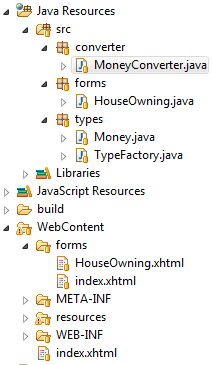
\includegraphics[width=5cm]{./images/chapter02/referenceimpl_forms.png}
\end{wrapfigure}

The questionnaire content basically consist of 3 main artifacts:

\begin{itemize}
\item \texttt{WebContent/forms/index.xhtml} - a link for each form will be
available here, it uses \texttt{WebContent/index.xhtml} as template and will be
the template for concrete forms in our application
\item \texttt{WebContent/forms/HouseOwning.xhtml} - this file will implement the
questionnaire form, it uses \newline\texttt{WebContent/forms/index.xhtml} as its
template
\item \texttt{src/forms/HouseOwning.java} - the so called
\emph{BackingBean}\footnote{\url{http://docs.oracle.com/javaee/5/tutorial/doc/bnaqm.html}}
which holds the state of a questionnaire form
\end{itemize}

Within the reference application there are 3 additional artifacts which can be
seen as some kind of utils:

\begin{itemize}
\item Money.java - a custom type that can be used in a bean
\item MoneyConverter.java - a custom converter which will be used to convert
values entered in web pages to custom types used in the bean and vise versa
\item TypeFactory.java - a Factory that creates any kind of complex types (e.g.
instances of custom type Money)
\end{itemize} 


\paragraph{Form} $\;$ \\
The form of our reference application consists of different areas where each
defines a single element of the questionnaire. Each question has a label and an
input element. Whenever the user changes a value of an input element the page should reload partly by using
AJAX\footnote{\url{https://en.wikipedia.org/wiki/Ajax\_(programming)}}.

In the following listings and screenshots you can see how the different parts
of the questionnaire are defined and how they are rendered. 

The following represents a question which can be answered by yes OR no. The
label and checkbox are grouped by using a so called \texttt{div} to create a close relation
between them.

\begin{lstlisting}[language=HTML]
<div class="ym-grid">

	<h:outputLabel styleClass="ym-g33 ym-gl"
		value="Did you sell a house in 2010?" />

	<h:selectBooleanCheckbox styleClass="ym-g50 ym-gl"
		id="chkHasSoldHouse" value="#{houseOwning.hasSoldHouse}">
		<f:ajax execute="chkHasSoldHouse"
				render="grp_hasSoldHouse_hasBoughtHouse" />
	</h:selectBooleanCheckbox>

</div>
\end{lstlisting}

The JSF \texttt{html:outputLabel} tag is rendered to a \texttt{HTML
label} tag on server side before the server responses on client requests. 

\begin{lstlisting}[language=HTML]
<label class="ym-g33 ym-gl">
Did you sell a house in 2010?
    </label>
\end{lstlisting}

The JSF \texttt{html:selectBooleanCheckbox} will be translated in a more complex
\texttt{HTML:input} tag. The most interesting thing is the action definition
\texttt{onclick} which lets JSF do some magic via AJAX to trigger partial page
reloads. The base functionality is provided by the JSF framework and some
JavaScript libraries.

\begin{lstlisting}[language=HTML]
<input id="houseOwningForm:chkHasSoldHouse" 
	class="ym-g50 ym-gl" type="checkbox"
	onclick="mojarra.ab(
				this,event,'valueChange','houseOwningForm:chkHasSoldHouse','houseOwningForm:grp_hasSoldHouse_hasBoughtHouse'
			)"
	checked="checked" 
	name="houseOwningForm:chkHasSoldHouse">
</input>
\end{lstlisting}
    
On client side the browser renders the question well grouped by use of some CSS
framework classes already mentioned in section \ref{sec:template}. 

\begin{center}
 
\includegraphics[width=10cm]{./images/chapter02/referenceimpl_forms_bool.png}
\end{center}

The following CSS classes out of
\texttt{WebContent/resources/default/css/base.css} are responsible for the shown
layout.

\begin{itemize}
  \item \texttt{ym-grid} - defines that childs should be grouped in a table
  \item \texttt{ym-g*number} - defines the width of an element
  \item \texttt{ym-gl} - defines that the element should float to the left of its
  container
\end{itemize}

Other question types are following the same pattern of a label and a proper
input element to interact with the application.

\begin{lstlisting}[language=XHTML]
<div class="ym-grid">

	<h:outputLabel styleClass="ym-g60 ym-gl"
		value="Price the house was sold for:" />

	<h:inputText styleClass="ym-g33 ym-gl" id="inSellingPrice"
		value="#{houseOwning.sellingPrice.amount}">
			<f:ajax event="keyup" execute="inSellingPrice"
				render="grp_ValueReside" />
	</h:inputText>

</div>
\end{lstlisting}

As you can see in the figure above the definition of an JSF
\texttt{html:inputText} tag is also very easy. With \texttt{\#\{\ldots\}} it is
possible to access a bean and its values. In our sample we access a property
\texttt{amount} of a property \texttt{sellingPrice} of a bean with name
\texttt{houseOwning}. :)

\begin{lstlisting}[language=HTML]
<input id="houseOwningForm:inSellingPrice" 
	class="ym-g33 ym-gl" 
	type="text"
	onkeyup="mojarra.ab(
				this,event,'keyup','houseOwningForm:inSellingPrice','houseOwningForm:grp_ValueReside'
			)"
	value="0" 
	name="houseOwningForm:inSellingPrice">
</input>
\end{lstlisting}

\begin{center}
 
\includegraphics[width=10cm]{./images/chapter02/referenceimpl_forms_text.png}
\end{center}

%\paragraph{Bean}





